% !TEX root = ../main.tex
% Chapter 4

\chapter{Proposed method}

\label{Chapter4} % For referencing the chapter elsewhere, use~\ref{Chapter4}

\lhead{Chapter 4. \emph{Proposed method}} % This is for the header on each page - perhaps a shortened title

%----------------------------------------------------------------------------------------
\section{Outline}
\emph{Not intented for the reader.}
\begin{itemize}
  \item Based on the problem statement with current research as stated in \Cref{Chapter3}
  \item Adjust method to needs
  \item Explain using graphs, pseudo-algorithms. Make clear distinction in origin of ideas and why to apply
\end{itemize}


\subsection{Experiment notes}
\begin{itemize}
  \item ICSS/CUSUM is goed in het vinden van variance changes. Niet goed in mean veranderingen.
  \item Problemen met SVM methode: ook na de verandering blijft de threshold nog stijgen;
  \item geprobeerd direct model-reset te doen na change point, maar dan kan je achteraf niet meer verder analyseren.
  \item Veranderingen in mean geven ``extra'' change point wanneer alle data weer in het window zit. Zie \Cref{fig:camci_fixed_increasing_mean} op de 50-tallen.
\end{itemize}


\begin{description}
  \item[Data gathering] Explain data gathering methods. Refer to chapter 5 and 6 for articifial and real-world details.
  \item[Model construction] Explain SVDD model construction and updating.
  \item[Model properties] Explain the SVDD properties that are used to calculate the change indication.
  \item[Change detection] Explain the interpretation of the properties, the possible (modulair) methods to give change indication
\end{description}


\TODO{Write chapter introduction/outline. Give overview of method approach and refer to each section for details of that stage.}

\TODO{Puts emphasis on two-stage framework by Takeuchi and Yamanishi \cite{takeuchi2006unifying}.}.

\begin{figure}
  \centering
    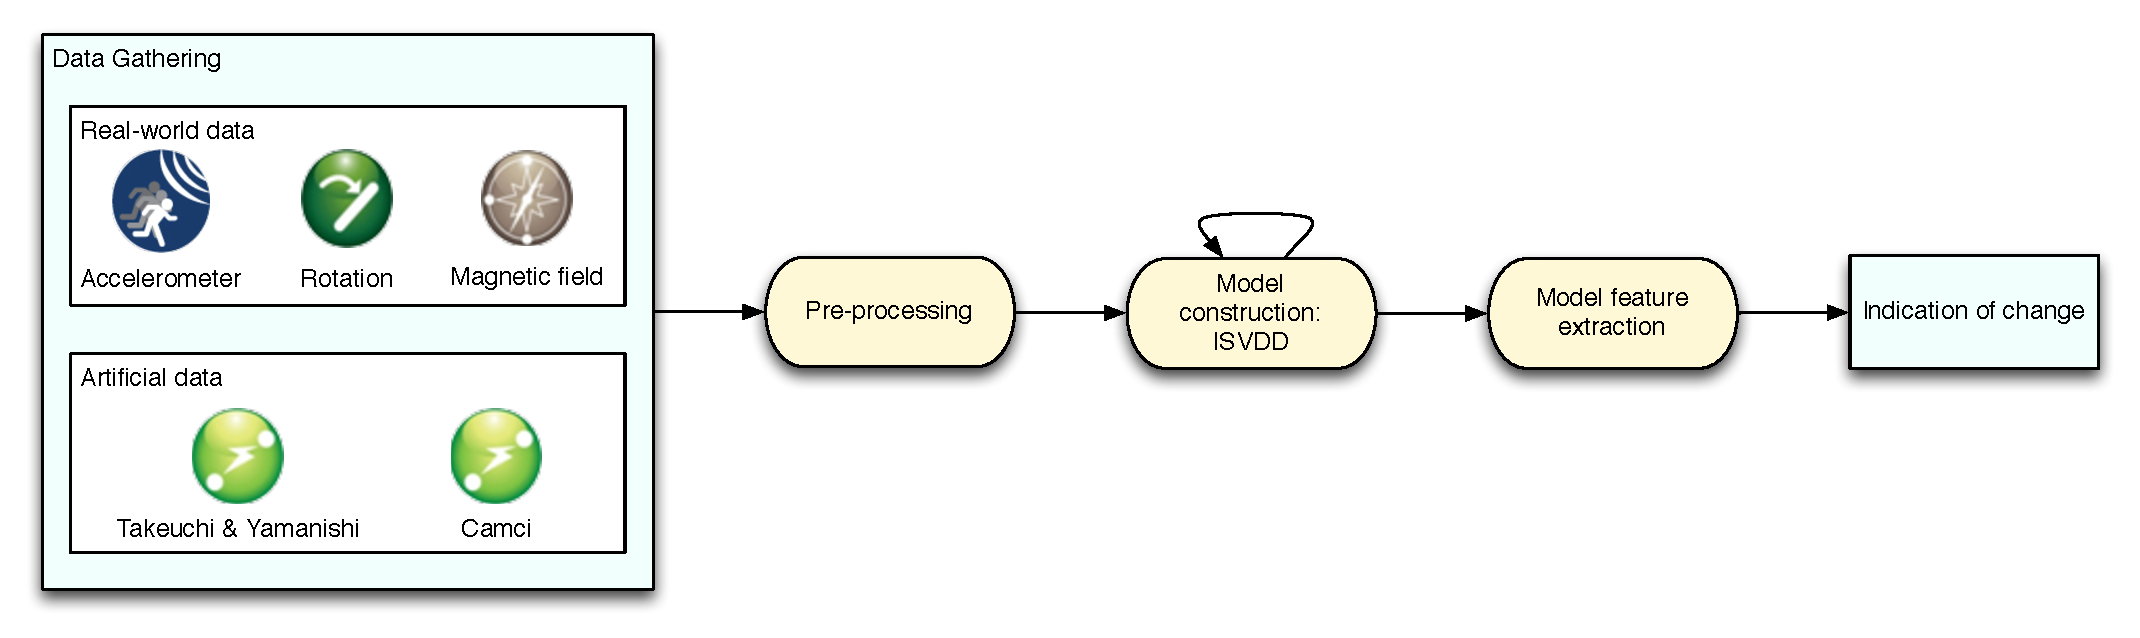
\includegraphics[width=\textwidth,height=\textheight,keepaspectratio]{./Figures/chapter4/method_setup_short.pdf}
  \caption[Method setup]{Schematic overview of the change detection method. The first step is the data gathering, described in Section \ref{sec:method_data_gathering}. Ater the pre-processing, the data is used to construct a \gls{svdd} model, as described in Section \ref{sec:method_model_construction}. Section \ref{sec:method_model_features} describes which features of the model are used for the final change indication algorithm, discussed in Section \ref{sec:method_change_detection}.}
  \label{fig:method_overview_short}
\end{figure}

% !TEX root = ../../main.tex
\section{Data Gathering}\label{sec:method_data_gathering}
In this section we briefly discuss the different data gathering methods used for the change detection algorithms and experiments.
\Cref{subsec:data_gathering_artificial} discusses the artificial data sets we will use.
In \Cref{subsec:data_gathering_real_world} an overview of the real-world data sets used is provided.
Both sections refer to Chapters~\ref{Chapter5} and~\ref{Chapter6} for more details, respectively.

% ------
\subsection{Artificial data}\label{subsec:data_gathering_artificial}
In order to provide an objective comparison to other methods, we will use artificial data sets which are also used in the earlier work on which \gls{ocs-hats} is based.
These are the data sets used by Takeuchi and Yamanishi \cite{takeuchi2006unifying} and Camci \cite{camci2010change}.
Both construct a collection of one-dimensional time series data according to a second order \gls{ar} model:
\begin{equation}
  x_t = a_1 x_{t-1} + a_2 x_{t-2} + \epsilon_t.
\end{equation}
Over the different data series the mean and variance of the Gaussian random variable $\epsilon_t$ differs and changes at pre-determined change points.
Using this data set an objective quality measure over the change detection methods can be obtained and compared.
All the used data sets are listed and analyzed in \Cref{Chapter5}.

% ------
\subsection{Real-world data}\label{subsec:data_gathering_real_world}
In the second type of data sets we apply our method for change detection and temporal segmentation to real-world data sets.
For our setup we record the activities of humans performed both in- and outdoor in an unknown environment.
Activities performed include sitting, standing, walking, running in a straight and curved line, and walking up- and downstairs.
\gls{ocs-hats} uses the signals from the accelerometer, magnetic field, and rotation sensors.
These time series data are used to detect change points.
A video recording from the performed activity is used to annotate the time series with real change points.
The discovered change points are compared with these annotated change points to give a subjective quality measure.
In \Cref{Chapter6} we give a detailed analysis of the performed activities and the recorded data sets.

For the experiments we used a smartphone with inertial sensors as recording device.
The activities were recorded using a free \textsc{Android} application \cite{sensorlogger}.
This application was chosen for its convenient data format of the sensor recording and its regularity of the sampling interval.
Table~\ref{tab:recorded_metrics} lists all the recorded metrics.
For our experiments we used the data for the accelerometer, magnetic field and rotation.

We implemented our algorithm in \textsc{Matlab}.
For the \gls{svdd} model construction phase we used the \textsc{dd\_tools} library by Tax \cite{Ddtools2013}, which depends on the \textsc{PR\_tools} package, originating from the book by Van Der Heijden \etal \cite{van2005classification}.
Alternatively, the widely used \textsc{LibSVM} \cite{chang2011libsvm} add-on for the \gls{svdd} algorithm by Chang \etal \cite{changrevisit} can be used.

\begin{center}\begin{table}
  \caption[Measured metrics]{Measured sensor metrics. The set of axis is always the triple (x, y, z) direction.}
  \begin{tabulary}{\textwidth}{|l|L|c|c|}
    \hline
    Sensor metric & Description & Units of measure & Typical range \\
    \hline \hline
    Accelerometer & Acceleration force along each axis (including gravity). & $m/s^2$ & $-20$ -- $20$ \\
    \hline
    Gravity & Force of gravity along each axis. & $m/s^2$ & $-10$ -- $10$\\
    \hline
    Gyroscope & Rate of rotation around each axis. & $rad/s$ & $-15$ -- $15$\\
    \hline
    Light & Light sensitive sensor at the front of the phone. & & $0$ -- $10000$ \\
    \hline
    Linear acceleration & Acceleration force along each axis (excluding gravity). & $m/s^2$ & $-20$ -- $20$ \\
    \hline
    Magnetic field & Geomagnetic field strength along each axis. & $\mu T$ & $-60$ -- $60$ \\
    \hline
    Orientation & Degrees of rotation around the three physical axis. & Degrees & $-100$ -- $360$ \\
    \hline
    Rotation & Measure of rotation around the device's rotation axis. & Unitless & $-1$ -- $1$\\
    \hline
  \end{tabulary}

  \label{tab:recorded_metrics}
\end{table}\end{center}

% !TEX root = ../../main.tex
\section{Model Construction: Incremental SVDD}\label{sec:method_model_construction}
After the data is collected and pre-processed (or in the case of the artificial data sets: generated), we construct an online incremental sliding window model construction algorithm.
We follow the method and implementation introduced by Tax and Laskov \cite{tax2003online}, the \acrlong{isvdd} method.
This method combines the techniques of online, unsupervised and incremental learning methods with the earlier introduced \gls{oc-svm} algorithm \gls{svdd}.
The method is first initialized with a window length and then in every step a new data object is added to and the last data object is removed from the working set.

Using the following abstract form of the \gls{svm} optimization problem, the extension of the incremental \gls{svm} to the \gls{svdd} can be carried out:
\begin{equation}
  \operatorname*{max}_\mu \operatorname*{min}_{\substack{
    0 \le x \le C \\
    \vectorsym{a}^T \vectorsym{x} + b = 0}
  } : W = -\vectorsym{c}^T\vectorsym{x} + \frac{1}{2}\vectorsym{x}^T K\vectorsym{x} + \mu(\vectorsym{a}^T\vectorsym{x} + b),
\end{equation}
where $\vectorsym{c}$ and $\vectorsym{a}$ are $n \times 1$ vectors, $K$ is a $n \times n$ matrix and $b$ is a scalar.
The \gls{svdd} implementation of this abstract form is set by the parameters $\vectorsym{c}=\operatorname*{diag}(K)$, $\vectorsym{a} = \vectorsym{y}$ and $b=1$.
The procedure for the incremental version has two operations: adding and removing a data object $k$.
When a data object $k$ added, its weight $x_k$ is initially set to $0$.
In case of an object removal, the weight is forced to be $x_k=0$.
Both the operations conclude with the recalculation $\mu$ and the weights $\vectorsym{x}$ for all the objects, in order to obtain the optimal solution for the enlarged or reduced data set.
The incremental learning algorithm follows from these two operations: new data objects are added to and old data objects are removed from the working set.

The size of the initial window of data objects has a lower bound determined by the hyperparameter $C$ (Equation \ref{eq:svdd_objective}).
Because of the equality constraint $\sum_{i=1}^n a_i x_i = 1$ and the box constraint $0 \le x_i \le C$, the number of objects in the working set must be at least $\ceil{\frac{1}{C}}$.
Thus the algorithm is initialized by selection the first $\ceil{\frac{1}{C}}$ objects for the working set.
In every step of the loop of the algorithm at least the same number of objects must be added as there are removed.
By analyzing the \gls{kkt} conditions, \cite{tax2003online} shows the optimality of the algorithm.

From experiments it shows that the online, \gls{isvdd}, method results in less false alarms than the static \gls{svdd}.
An explanation for this is that \gls{isvdd} follows the changing data distribution, such that small changes over time, like a drift in mean or increase in frequency, continuously re-model the \gls{svm} representation.
% !TEX root = ../../main.tex
\section{Model Features}\label{sec:method_model_features}
In the previous section we have discussed the \gls{isvdd} method, which creates a \gls{oc-svm} representation of a working set of data objects at every step of the algorithms loop.
This section shows how we interpret the constructed model and extract features to obtain a measure which can be used for an indication of change points.
The next section discusses how this obtained measure is used to indicate change.

The \gls{isvdd} algorithm creates a spherical \gls{oc-svm} representation of the working set at every step of the algorithm.
This model is obtained by the minimization of \Cref{eq:svdd_objective}, which incorporates the radius $R$ of the sphere and the distances $\vectorsym{\xi}$ from the outliers to the boundary.
We will use the radius $R$ of the hypersphere as an indication of change.

In \cite{tax2002uniform} Tax and Duin provide an analysis of the error of the \gls{svdd} algorithm.
This error is based on
\begin{inparaenum}[\itshape 1\upshape)]
\item the fraction $f_{T-}$ of target objects that is rejected, and
\item the fraction $f_{O+}$ of outliers that is accepted.
\end{inparaenum}
Since in \gls{occ} situations typically there are (almost) no examples of outlier objects, Tax and Duin construct a method to generate outliers based on the assumption that the the location of (potential) outliers are uniformly distributed around the target set.
To minimize the error, calculated by the fractions $f_{T-}$ and $f_{O+}$, we should minimize the volume of the target data description (\ie the boundary of \gls{svdd}).
That is because the fraction of accepted outliers $f_{O+}$ is an estimate of the volume of the target data description, with respect to the volume of the outlier distribution.
Tax and Duin provide a method to optimize the parameters of the \gls{svdd} method, \ie the trade-off parameter $C$ and the \gls{rbf} kernel width $\sigma$.
This optimization will result in the modification of the radius $R$ of \Cref{eq:svdd_objective} and affects the Lagrangian inequality~(\ref{eq:svdd_inequality}).

\begin{figure}
  \centering
    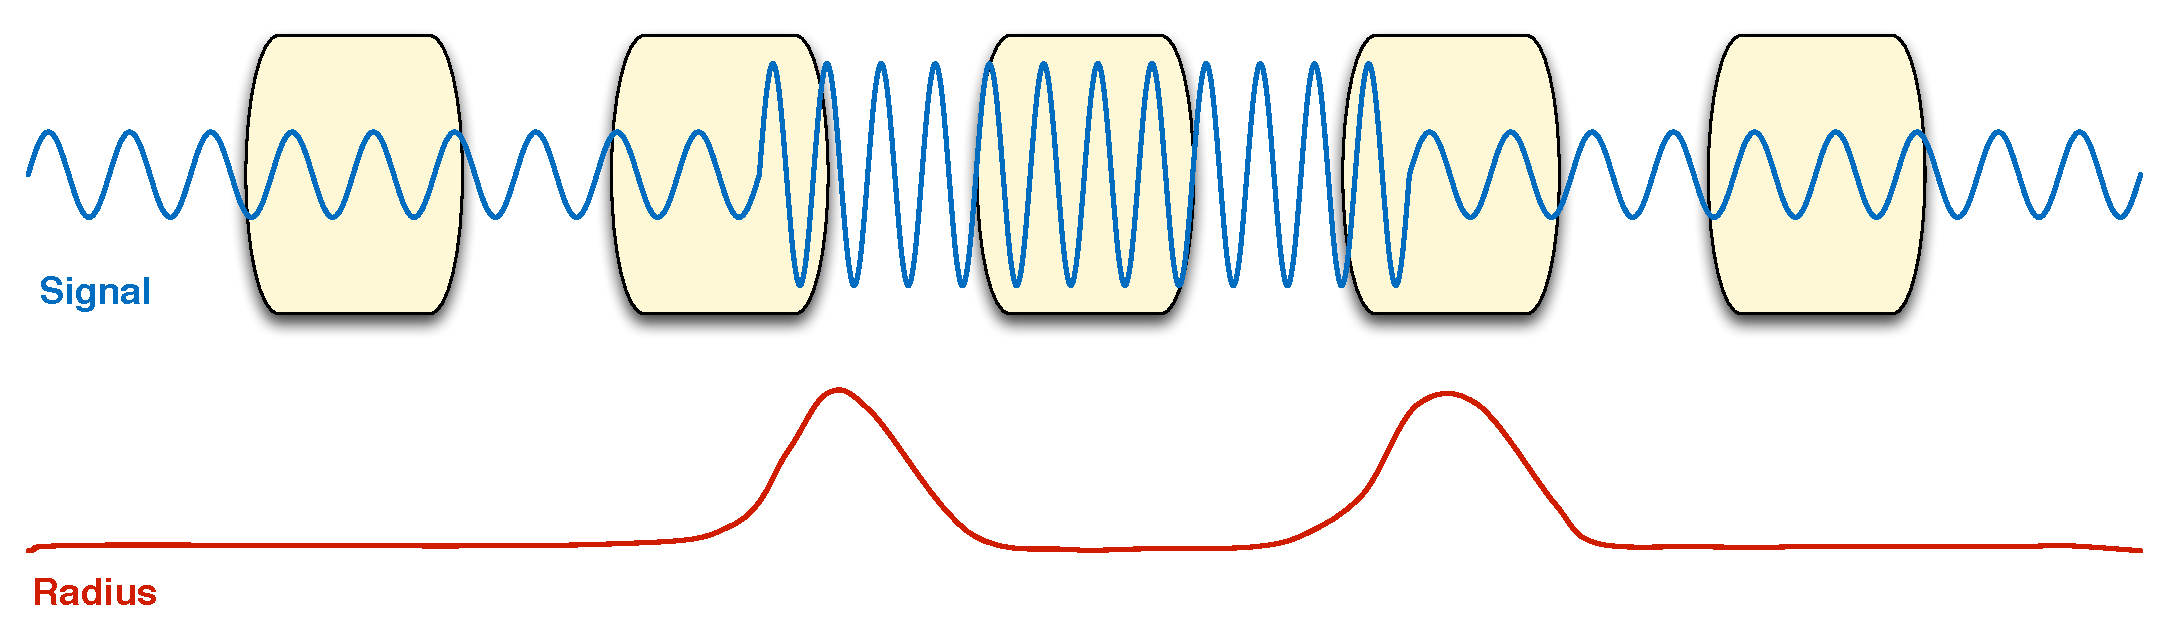
\includegraphics[width=\textwidth,height=\textheight,keepaspectratio]{./Figures/chapter4/expected_behaviour.pdf}
  \caption[Expected radius behavior]{Expected behavior of the radius $R$ of the hypersphere. The upper part shows a typical sinusoidal time series signal. The lower graph visualizes an abstract expectation of the values of $R$. Five possible time windows are illustrated. Windows $a$, $c$ and $e$ cover an area of homogeneous signal. The expected value of $R$ is low. The other two windows, $b$ and $d$ cover a change entering and leaving the window, respectively. At these locations the radius $R$ is expected to increase temporarily.}
  \label{fig:radius_expectation}
\end{figure}

Since in our method the parameters $C$ and $\sigma$ are kept constant, and thereby also the fraction of target objects being rejected, the only free parameter is the radius $R$.
During the \gls{isvdd} algorithm the volume of the hypersphere is minimized.
This means that only the radius of the sphere will change during the analysis over the time series data.
We will interpret changes in the radius $R$ with the same continuity assumptions as mentioned in \Cref{subsec:kernels}.

For instance, consider two hyperspheres that model two different, but partially overlapping, working sets of objects.
If the radius size of these two hyperspheres are close to each other, that means the distribution of objects in the sets are also similar.
In other words, if the distribution over objects in a working set changes, so does the characteristics of the set, and the radius $R$ of the hypersphere will also change.
If in the case of a change in distribution the data objects in the working set become more heterogeneous, the radius of the hypersphere will increase.
When, instead, the data objects change from a heterogeneous set to a more homogeneous, we expect the radius to decrease in value, since the data objects are closer to each other in the feature space.
This relation between the signal and expected radius $R$ is illustrated in \Cref{fig:radius_expectation}.
It shows that in the two time windows that cover a heterogeneous set of data objects, the radius of the hypersphere is expected to be relatively high.

With the \gls{isvdd} algorithm we have effectively implemented a form of dimensionality reduction by feature extraction, using the radius $R$.
The following section discusses the algorithms which can be applied to the extracted radius $R$ as a volume estimate.
We thereby follow the setup of the unifying framework by Takeuchi and Yamanishi~\cite{takeuchi2006unifying}, of which this section described the first stage.
% !TEX root = ../../main.tex
\section{Change Detection}\label{sec:method_change_detection}

 % --- OLD ---
% % !TEX root = ../../main.tex
\section{Change Indication}\label{sec:method_change_indication}
*** TODO: change section title ***
*** TODO: ***
\emph{Follow methodology of ``A unifying framework for detecting outliers and change points from time series'' \cite{takeuchi2006unifying}.
It creates a two-stage process of first searching for outliers, and then using the ``outlier-score'' to find (sudden) change points, by a weighted average of a moving window.
That eventual score can be thresholded (as in the paper) or processed with something like CUSUM (proposal).
Looks like my proposed methods, in that is combines outliers and gives a score to change points.}

The proposed method of this thesis follows the unifying framework as introduced by Takeuchi and Yamanishi \cite{takeuchi2006unifying} and an similar implementation by Camci \cite{camci2010change} with \glspl{svm}.
The unifying framework combines the detection of outliers with change points and divides it in two stages.
The first stage determines the outliers in a time series by giving a score based on the deviation from a learned model, and thereby creates a new time series.
The second stage runs on that new created time series and calculates a average over a window of the outlier scores.
The problem of change detection is then reduced to outlier detection over that average-scored time series.
This method is named \gls{changeFinder} by the authors.
The implementation by Camci, which uses \glspl{svm} to detect changes is named \acrlong{svcpd}.

The problem statement and formal definition, following Tackeuchi and Yamanishi \cite{takeuchi2006unifying} and Camci \cite{camci2010change} is the following.
The algorithm needs to find \emph{sudden} changes in the time series data.
In other words, slowly changing properties in the data are not considered to be changes.
This is in line with the search of changes in activities, since we are only interested in different activities (which are represented by sudden changes) instead of changes within an activity.
Considered a time series $x_1 x_1 \dots$, which is drawn from a stochastic process $p$.
Each $x_t$ (t = 1, 2, \dots) is a $d$-dimensional real valued vector and $p$ a probability density function of the sequence $x_1 x_2 \dots$.
Assume $p$ can be decomposed in two different \gls{iid} stationary stochastic processes $p^1$ and $p^2$ and are one-dimensional Gaussian density functions.
For a time point $a$ data points for which $t < a$ are drawn from $p^1 = N(\mu_1, \sigma_1^2)$ and for $t \geq a$ from $p^2 = N(\mu_2, \sigma_a^2)$.
If $p^1$ and $p^2$ are different, then the time point $t = a$ is a \emph{change point}.
In \cite{takeuchi2006unifying} the similarity between the stochastic processes are expressed by the \gls{kliep} divergence $D(p^2||p^1)$.
The problem with this measure is that, as the authors conclude and Camci discusses, it is not able to detect a change by decrease in variance.

Whereas \gls{changeFinder} uses double probability estimation algorithm, our approach follows \gls{svcpd} by constructing a \gls{svm} over a sliding window.
The \gls{svcpd} algorithm uses the location of new data points in the feature space $\mathcal{F}$ with respect to the hypersphere and the hypersphere's radius $R$ to determine whether the new data point represents a change point.

*** TODO: What is my contribution compared to Camci? Distance of outliers to hypersphere? ***
% % !TEX root = ../../main.tex
\section{Overview}\label{sec:method_overview}

\begin{figure}
  \centering
    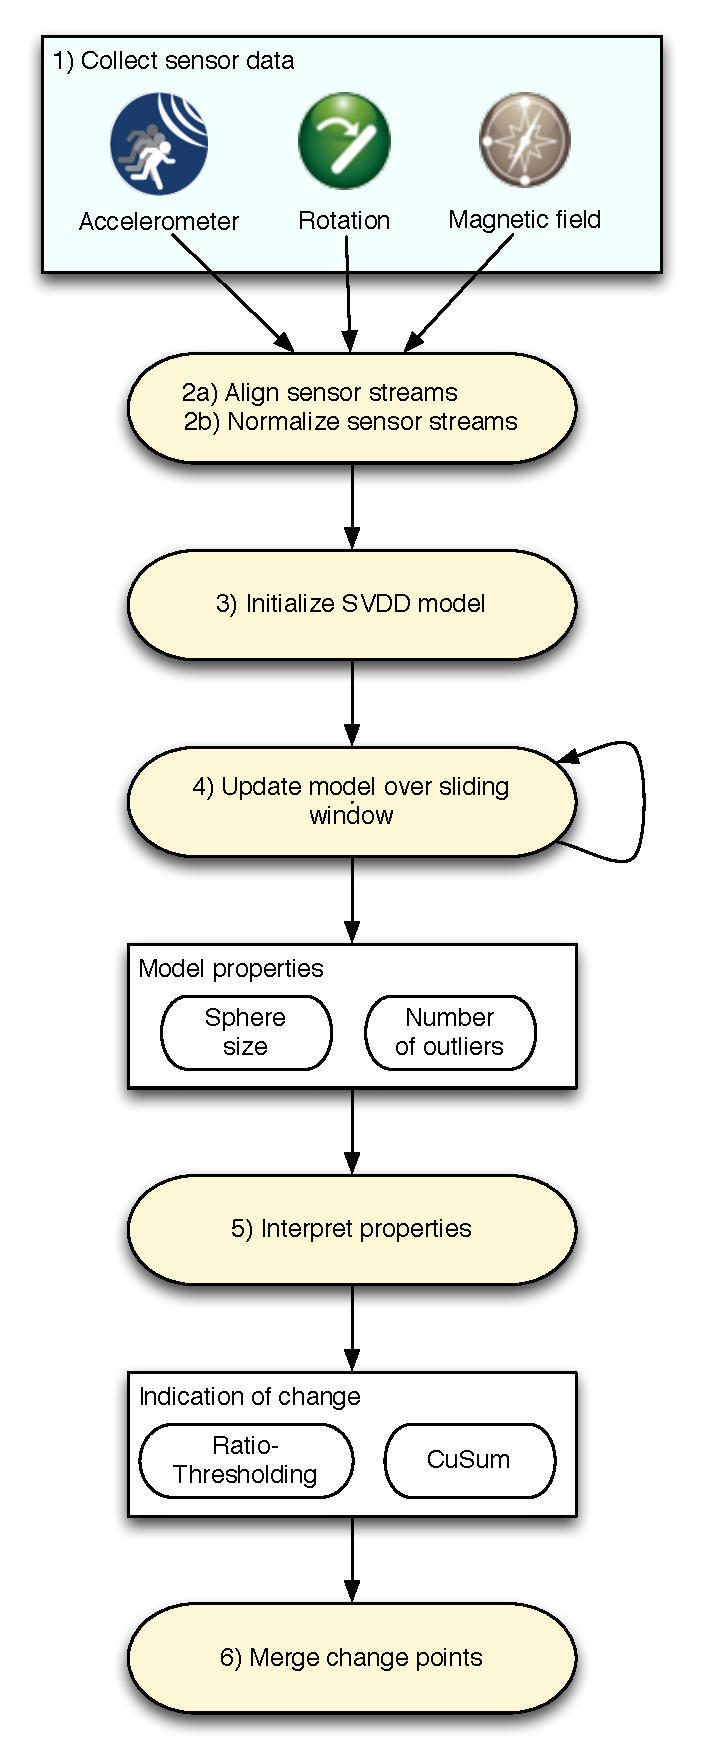
\includegraphics[width=\textwidth,height=\textheight,keepaspectratio]{./Figures/graphs/chapter4/method_setup.pdf}
  \caption[Method setup]{Schematic representation of the change detection method.}
  \label{fig:method_overview}
\end{figure}

This section gives a description of the method used for the experiments and change detection mechanism.
First described is the method to process the gathered sensor data.
A schematic overview is given in figure \ref{fig:method_overview} and shows the steps of the method.
A more detailed explanation of the ``Update model'' step follows.
This section is finalized with the experiments setup, annotation of data streams and quality measure.

\subsection{Change detection method}
As graphically represented in figure \ref{fig:method_overview}, the change detection method starts by processing the data from sensor, such as the accelerometer, magnetic orientation and rotation measures \footnote{Something about the origin of the streams; all from the same sensor or different sensors?}.

The first step is to process the raw streams of data originating from a multiple of sensors.
The two processes applied are alignment and normalization.
Due to noisy sampling, not all the timestamps in the data streams are sensed at the same timestamp.
Since the \gls{svdd} method requires all the data stream at every timestamp and can not handle missing data on one of the timestamps, all the unique timestamps are filtered out.
Whilst this results in an overall filtering effect, in practice between $1\%$ and $5\%$ of each data stream is disregarded.
The effect of this filtering is not significant and the data is not modified.

Due to the nature of the sensor signals, a normalization step is required in order to set the weight for all the data streams equal.
The range of the accelerometer signal typically spans $-20$ to $20$, the magnetic field from $-60$ to $60$ and the rotations range is from $-1$ to $1$.
This means that a relative small change in the accelerometer stream could have a much larger impact on the model than the same (absolute) change in the rotation stream, whilst the latter has a larger relative impact.
The normalization step ensures that all data is weighted equally and changes in the data are all proportional.

In step $3$ the \gls{svdd} model is initialized.
The first full window over the data stream is used to construct an initial model.
During the initialization the parameters for the \gls{svdd} are provided, begin the kernel type (radial), \gls{rbf} with $\sigma$ and the outlier-fraction $C$.

Step $4$ is executed for every step-size $s$ data points in the stream.
Every update the oldest $s$ data points are removed from and $s$ new data points are added to the \gls{svdd} model.
The model is (partially) reconstructed and new model properties, such as the radius of the hypersphere and the number of outliers, are the result of this step \footnote{Other measures are also possible, for instance the distance from all the outliers to the boundary of the hypersphere}.
*** MORE ON THE UPDATING STEP ***

This final step of this method, step $5$, is the interpretation of the model properties.
Many algorithms can be used for this process, all which take a one-dimensional time series as input and determine where change has occured.
In our setup we used the \gls{rt} and \gls{cusum} methods, to show the modularity of this step.

\subsection{Model updating}

\subsection{Experiments}
For the experiments we used a HTC Sensation XE smartphone as recording device.
The activities were recorded using a free Android application \cite{sensorlogger}.
This application was chosen for its convenient data format of the sensor recording and its regularity of the sampling interval.
Table \ref{tab:recorded_metrics} lists the recorded metrics.
For our expiments we used the data for the accelerometer, magnatief field and rotation.

\begin{center}\begin{table}
  \begin{tabulary}{\textwidth}{|l|L|c|c|}
    \hline
    Metric & Description & Units of measure & Typical range \\
    \hline \hline
    Accelerometer & Acceleration force along each axis. & $m/s^2$ & $-20$ -- $20$ \\
    \hline
    Gravity & Force of gravity along each axi.s & $m/s^2$ & $-10$ -- $10$\\
    \hline
    Gyroscope & & $rad/s$ & $-15$ -- $15$\\
    \hline
    Light & Light sensitive sensor at the front of the phone. & & $0$ -- $10000$ \\
    \hline
    Linear acceleration & & $m/s^2$ & $-20$ -- $20$ \\
    \hline
    Magnetic field & Geomagnetic field strength along each axis. & $\mu T$ & $-60$ -- $60$ \\
    \hline
    Orientation & & & $-100$ -- $360$ \\
    \hline
    Rotation & & & $-1$ -- $1$\\
    \hline
  \end{tabulary}
  \caption{Measured metrics. The set of axis is always the triple (x, y, z) direction.}
  \label{tab:recorded_metrics}
\end{table}\end{center}

